\documentclass[12pt,a4paper]{article}
\usepackage{rmpackages}																% usual packages
\usepackage{rmtemplate}																% graphic charter
\usepackage{rmexocptce}																% for DS with cptce eval

%\cfoot{} 													% if no page number is needed
\renewcommand\arraystretch{1.}		% stretch table line height

\begin{document}

\begin{header}
Interrogation -- Chapitre 6

\normalsize
\flushleft
\begin{doublespace}
Classe :

NOM :

\end{doublespace}
Prénom : 
\end{header}

\emph{La formule littérale et, si cela est nécessaire, le détail des conversions sont attendus chaque fois qu'un calcul est requis pour répondre à la question.}

\begin{exo}{Catapultage d'un avion de chasse}

\begin{multicols}{2}
\begin{center}
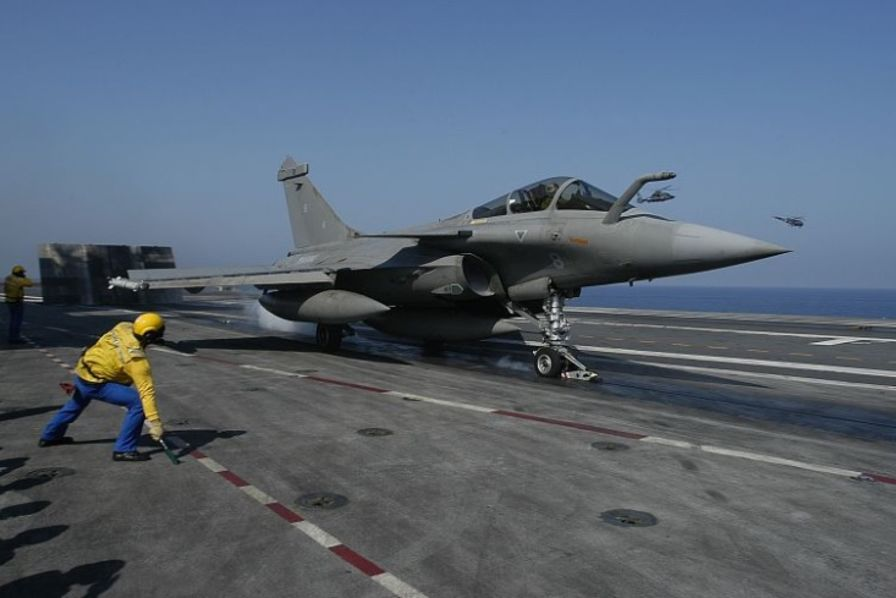
\includegraphics[trim={0 4cm 0 4cm}, clip, width=\linewidth]{images/rafale.jpg}
\end{center}

Pour faire décoller un avion de chasse depuis le pont d'un porte-avion, on utilise un système de catapulte qui lui permet d'atteindre rapidement une vitesse suffisante.
Le pilote passe ainsi de $0$ à \unit{250}{km/h} en \unit{2}{s} seulement !

Catapultage d'un rafale depuis le Charles de Gaulle : \href{https://youtu.be/gW4uZVK9hWU}{https://youtu.be/gW4uZVK9hWU}.
\end{multicols}

\begin{enumerate}
\item \app{} \ajapp{0.5}

Préciser le système étudié.

\item \anarai{} \ajanarai{0.5}

Indiquer le référentiel choisi dans la vidéo pour suivre le mouvement.
\end{enumerate}

Le schéma ci-dessous est une chronophotographie de l'avion lors du décollage.
Les positions de l'avion sont relevées toutes les \unit{0{,}4}{s}.
Le schéma est à l'échelle 1/1000 : \unit{1}{cm} sur le schéma = \unit{10}{m} en vrai.

\begin{center}
\begin{tikzpicture}

\foreach \t in {0, 1, ..., 5} {
  \newcommand{\temps}{\t/2.5}
  \draw (3.5*\temps*\temps/2, 0) node {$\bullet$};
   \coordinate (F) at (3.5*\temps*\temps/2, 0);
}
\draw (0,0) node [above left] {$M_0$};
\foreach \t in {1, 2, ..., 5} {
  \newcommand{\temps}{\t/2.5}
  \draw (3.5*\temps*\temps/2, 0) node [above] {$M_\t$};
}

\draw (F) ++ (5:7*.4) node {$\bullet$} ++ (10:7*.4) node {$\bullet$} ++ (15:7*.4) node {$\bullet$};
\draw (F) ++ (5:7*.4) node [above] {$M_6$} ++ (10:7*.4) node [above] {$M_7$} ++ (15:7*.4) node [above] {$M_8$};

\draw [<->, >=stealth, bleu_f] (0,-.5) -- (7.5,-.5) node [midway, below] {catapultage};
\draw [<-, >=stealth, red_f] (7.5,-.5) -- (15,-.5) node [midway, below] {vol};
\draw [dashed, red_f] (15,-.5) -- (15.5,-.5);

\end{tikzpicture}
\end{center}

\begin{enumerate}[resume]
\item \rco{} \ajrco{1}

Décrire le mouvement de l'avion lors du catapultage, c'est-à-dire entre les points $M_0$ et $M_5$ (trajectoire et vitesse).

\item \rco{} \ajrco{0.75} \anarai{} \ajanarai{0.75}

Rappeler les caractéristiques du vecteur vitesse.
Comment évoluent-elles pendant le catapultage ?

%\item \rco{}

%Décrire le mouvement de l'avion après le décollage, c'est-à-dire après $M_5$ (trajectoire et vitesse).

\item \rea{} \ajrea{2}

Représenter sur la chronophotographie le vecteur vitesse $\vec{v_6}$ juste après le décollage, en $M_6$.
On prendra comme échelle pour représenter le vecteur vitesse $\unit{1}{cm} \leftrightarrow \unit{20}{m/s}$.

\item \rea{} \ajrea{0.5} \val{} \ajval{0.5}

La valeur de la vitesse trouvée précédemment vous semble-t-elle cohérente ?

\item \rea{} \ajrea{1}

Une fois en vol, ces avions peuvent parcourir jusqu'à \unit{3700}{km} en seulement \unit{3}{h}.
Calculer la vitesse moyenne de ces avions, en km/h, d'après ces valeurs.
\end{enumerate}

\end{exo}

\begin{exo}{Un classique}

\begin{multicols}{2}
\begin{enumerate}
\item \anarai{} \ajanarai{0.5}

Indiquer le référentiel le plus adapté à l'étude du mouvement de la Terre autour du Soleil.

\item \rco{} \ajrco{0.5}

Identifier les termes qui permettent de qualifier le mouvement de la Terre autour du Soleil :
\emph{rectiligne ; circulaire ; curviligne ; uniforme ; accéléré ; décéléré.}
\end{enumerate}

\begin{center}
\begin{tikzpicture}
\draw (0,0) node [yellow_f] {$\bullet$};
\draw (0,0) node [yellow_f, above] {Soleil};
\foreach \x in {0,30,...,360} {
  \draw (\x-20:2) node [color=bleu_f] {$\bullet$};
}
\draw (40:2) node [bleu_f, above right] {Terre};
\draw [color=bleu_f, dashed] plot [domain=0:360, smooth] (\x-20:2);
\draw [color=bleu_f, ->, >=stealth] plot [domain=20:50, smooth] (\x:1.5);
\end{tikzpicture}
\end{center}
\end{multicols}

\begin{enumerate}
\setcounter{enumi}{2}
\item \rco{} \ajrco{0.5}

Sans soucis d'échelle, représenter les positions successives d'un système ayant un mouvement rectiligne décéléré.
Préciser le sens du mouvement par une flèche.
\end{enumerate}

\end{exo}

\begin{exo}{Configuration électronique}

\begin{enumerate}
\item \anarai{} \ajanarai{0.5} \com{} \ajcom{0.5}

L'atome de silicium, de symbole Si, a un numéro atomique $Z=14$.
Indiquer, en le justifiant, le nombre d'électrons qu'il possède.

\item \anarai{} \ajanarai{1}

Écrire sa configuration électronique fondamentale.
\end{enumerate}

\end{exo}

\vfill
\makecptces{}

\end{document}

\newcommand{\step}{2.4}
\newcommand{\angl}{10}
\draw (0,0) node {$\bullet$} ++ (\angl:\step) node {$\bullet$} ++ (\angl/2:\step) node {$\bullet$} ++ (-\angl/2:\step) node {$\bullet$} ++ (-\angl:\step) node {$\bullet$} ++ (-\angl:\step) node {$\bullet$} ++ (-\angl/2:\step) node {$\bullet$} ++ (\angl/2:\step) node {$\bullet$} ++ (\angl:\step) node {$\bullet$};

\draw (0,0) [above right] node {$M_0$} ++ (\angl:\step) node {$M_1$} ++ (\angl/2:\step) node {$M_2$} ++ (-\angl/2:\step) node {$M_3$} ++ (-\angl:\step) node {$M_4$} ++ (-\angl:\step) node {$M_5$} ++ (-\angl/2:\step) node {$M_6$} ++ (\angl/2:\step) node {$M_7$} ++ (\angl:\step) node {$M_8$};